\documentclass{article}
\usepackage[T1]{fontenc}
\usepackage{lmodern}
\usepackage{graphicx}
\usepackage{amsmath,amssymb}
\usepackage[a4paper,margin=2cm]{geometry}
\usepackage[absolute,overlay]{textpos}
\setlength{\TPHorizModule}{1mm}
\setlength{\TPVertModule}{1mm}
\usepackage[indonesian]{babel}
\usepackage{hyperref}
\setlength{\emergencystretch}{2em}
% unit: Halaman 46

\begin{document}

% === Halaman 46 (llm) ===

\vspace{238.79mm}

Sejarah kriptanalisis mencatat hasil gemilang seperti pemecahan Telegram Zimmermann yang membawa Amerika Serikat ke kancah Perang Dunia I.\vspace{20mm}
\textcolor{red}{Telegram Zimmerman yang sudah berhasil didekripsi (Sumber: Wikipedia.org)}

% deskripsi: Screenshot dokumen Telegram Zimmermann yang telah didekripsi dalam bahasa Inggris.
% bbox normalisasi: [0.0600, 0.1080, 0.9400, 0.9120]
\begin{textblock*}{184.80mm}(12.60mm,32.08mm)
\noindent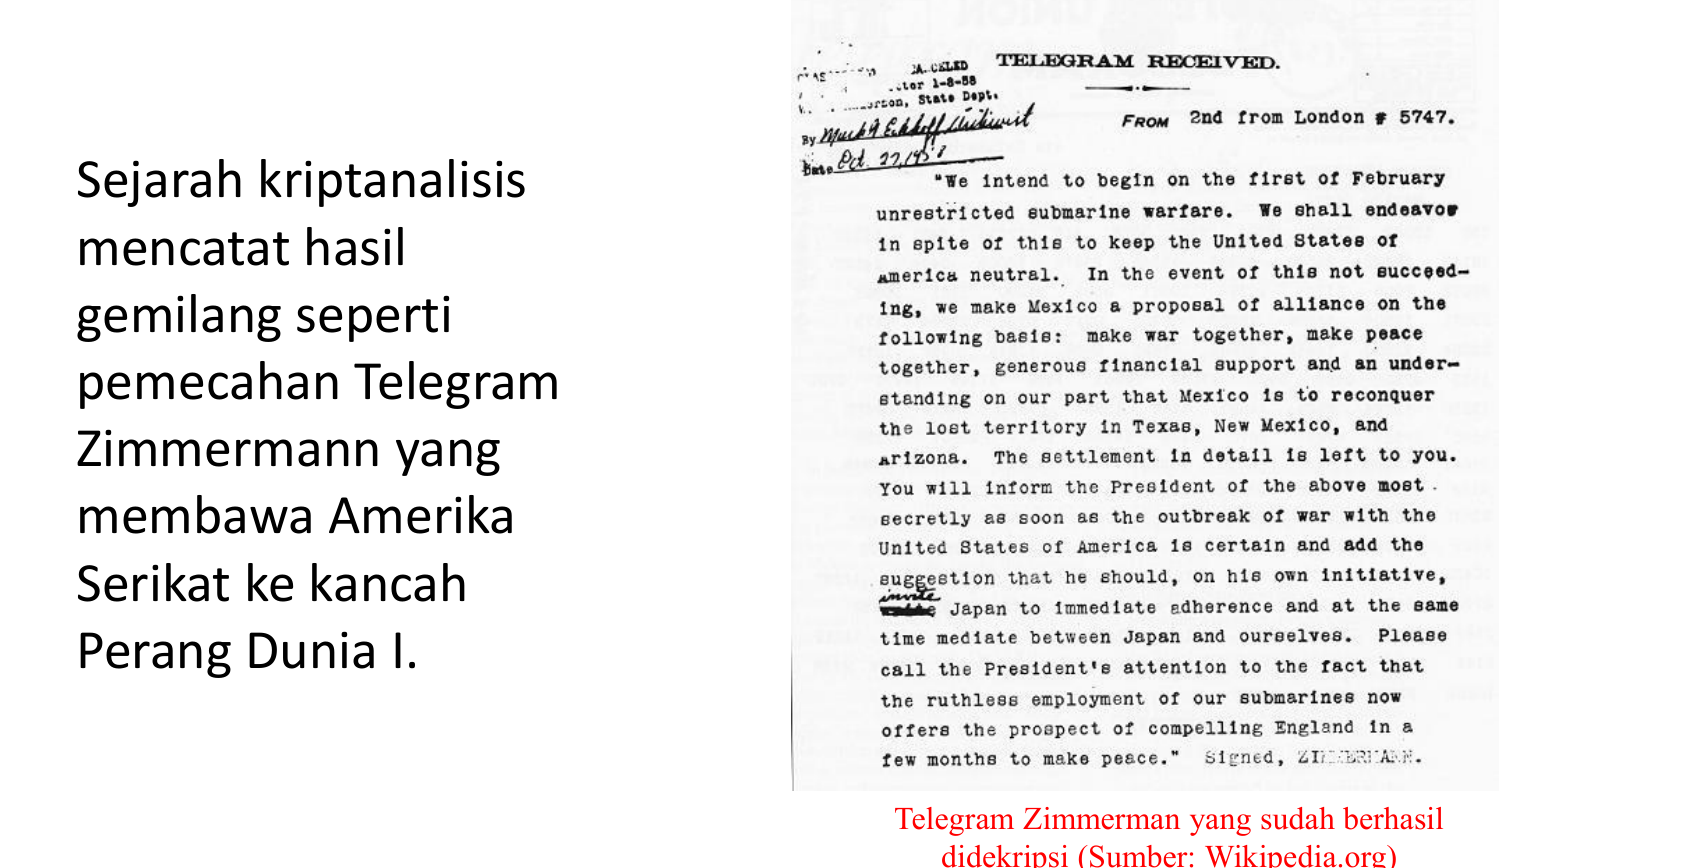
\includegraphics[width=184.80mm,height=238.79mm]{../../images/llm/page_046_img_01.png}%
\end{textblock*}

% bbox perkiraan otomatis: Screenshot dokumen Telegram Zimmermann yang telah didekripsi dalam bahasa Inggris.

\end{document}
